% TEMPLATE for Usenix papers, specifically to meet requirements of
%  USENIX '05
% originally a template for producing IEEE-format articles using LaTeX.
%   written by Matthew Ward, CS Department, Worcester Polytechnic Institute.
% adapted by David Beazley for his excellent SWIG paper in Proceedings,
%   Tcl 96
% turned into a smartass generic template by De Clarke, with thanks to
%   both the above pioneers
% use at your own risk.  Complaints to /dev/null.
% make it two column with no page numbering, default is 10 point

% Munged by Fred Douglis <douglis@research.att.com> 10/97 to separate
% the .sty file from the LaTeX source template, so that people can
% more easily include the .sty file into an existing document.  Also
% changed to more closely follow the style guidelines as represented
% by the Word sample file. 

% Note that since 2010, USENIX does not require endnotes. If you want
% foot of page notes, don't include the endnotes package in the 
% usepackage command, below.

% This version uses the latex2e styles, not the very ancient 2.09 stuff.
\documentclass[letterpaper,twocolumn,10pt]{article}
\usepackage{usenix,epsfig,endnotes}
\usepackage{amsmath,amsfonts,amssymb}
\usepackage{color}
\usepackage{mathtools}
\usepackage{graphicx}
\usepackage{url}
\usepackage{listings}
\usepackage[linesnumbered,ruled]{algorithm2e}

%\usepackage{algorithm}
\usepackage[noend]{algpseudocode}
\usepackage[utf8]{inputenc}
\usepackage[english]{babel}
\usepackage{amsthm}

\newcommand{\floor}[1]{\lfloor #1 \rfloor}
\DeclareMathOperator{\sign}{sign}
\makeatletter
\def\BState{\State\hskip-\ALG@thistlm}
\makeatother

\newtheorem{theorem}{Theorem}[section]


\theoremstyle{definition}
\newtheorem{definition}{Definition}[section]

\newcommand{\red}[1]{\textcolor{red}{#1}}

\begin{document}

%don't want date printed
\date{}

%make title bold and 14 pt font (Latex default is non-bold, 16 pt)
\title{\Large \bf LargeLSH: An Exploration of Locality Sensitive 
Hashing for Approximate Nearest Neighbours on High Dimensional Data Using Apache 
Spark}

%for single author (just remove % characters)
\author{
{\rm Wei\ Yang}\\
University of Waterloo
\and
{\rm Zhucheng Tu}\\
University of Waterloo
% copy the following lines to add more authors
% \and
% {\rm Name}\\
%Name Institution
} % end author

\maketitle

% Use the following at camera-ready time to suppress page numbers.
% Comment it out when you first submit the paper for review.
\thispagestyle{empty}


\subsection*{Abstract}

Nearest neighbour algorithms are a popular class of algorithms in machine learning 
that has a wide range of applications. When the dimensionality of the data is 
small, data structures from computational geometry can be used  
for efficiently finding nearest neighbours. However, when the dimensionality of the 
data is large, the space requirement of these data structures hinder them from 
being used in practice. Today, many internet companies store high dimensional 
features for their business entities, and it is not reasonable to assume all the 
data are stored on the same machine. We explore the problem of approximate nearest 
neighbour search in a distributed setting, specifically looking at the 
effectiveness of locality sensitive hashing (LSH) for this problem on high 
dimensional data. We find that \red{ipsum...}


\section{Introduction}

The problem of finding nearest neighbours has important applications in many areas. 
Finding the 
nearest neighbours means finding the nearest points to some reference point defined 
by some distance metric in some space. For example, e-Commerce websites might want 
to find the nearest neighbours of a product to recommend similar products to 
consumers for its recommender system, and financial institutions might want to find 
nearest neighbours of an account that performs fraudulent activities to identify 
similarly suspicious accounts. Some areas in computer science which the nearest 
neighbour problem is important include databases and data mining 
\cite{berkhin2006survey}, information retrieval \cite{croft2010search}, image and 
video databases \cite{faloutsos1994efficient,flickner1995query}, and machine 
learning \cite{weinberger2006distance}. \\

If the data set is of size $n$, and each data point is of dimension $d$, a naive 
approach would involve at looking at all the points in the entire data set and 
finding the nearest neighbours, a computation that has runtime of $\Theta(nd)$. 
Using data structures from computation geometry, we can reduce this to 
$\Theta(d\log(n))$, but the space complexity is $n^{O(d)}$, which is infeasible for 
high-dimensional data \cite{shalev2014understanding}. To avoid this ``curse of 
dimensionality", we can look toward approximate nearest neighbours, which is 
guaranteed to be within some distance bound of the true nearest neighbour 
(mathematically defined in next section). Some ways to tackle the approximate 
nearest neighbour problem include k-d trees, balltrees, and locality sensitive 
hashing (LSH) \cite{shakhnarovich2006nearest}. \\

Amidst the decreasing storage cost and the increasing popularization of cloud 
computing and big dat\textbf{a, }we can no longer assume that the high dimensional feature 
vectors of the data set can fit into the memory of one machine. For example, the 80 
million tiny images data set for object and scene recognition is 240 GB, far larger 
than the available memory of a usual computer \cite{torralba200880}. Many 
organizations also store their data in distributed file systems, such as the Hadoop 
Distributed File System (HDFS) \cite{shvachko2010hadoop}. MapReduce 
\cite{dean2008mapreduce} and Apache Spark \cite{zaharia2010spark} have become the 
de-facto distributed computation frameworks for massive parallel computation on 
large data sets \cite{suri2011counting}. \\

Given the importance of finding nearest neighbours and the proliferation of Spark, 
it makes sense to investigate the application of Spark to the approximate nearest 
neighbour (ANN) problem. Specifically, we focus on LSH using Spark, since LSH is an 
extremely simple method that can scale to high-dimensional data. LSH for Spark is 
an active area, since the LHS module only became available in Spark in December 
2016. 
\footnote{https://databricks.com/blog/2017/05/09/detecting-abuse-scale-locality-sensitive-hashing-uber-engineering.html}
  Previously it had to be implemented from scratch using the fundamental parallel 
  data processing constructs. We investigate the effect of parameters on the 
  accuracy versus running time tradeoff, the scalability of the Spark 
  implementation of LSH, and compare it to an open-source Spark spill tree 
  approach. \\


\section{Background and Related Work}

We first formally define the nearest neighbour problems.

\begin{definition}[Nearest Neighbour]
	
	Given a  point set $P \in \mathbb{R}^{n \cdot d}$, for any query point $q \in 
	\mathbb{R}^d$, return the $p \in P$ minimizing $\| p-q \|$, i.e. we wish to 
	find the point closest to $q$ by some metric.
	
\end{definition}

\begin{definition}[$(1 + \epsilon)$-Approximate Nearest Neighbour]
	Given a  point set $P \in \mathbb{R}^{n \cdot d}$, for any query point $q \in 
	\mathbb{R}^d$, if $p \in P$ satisfies
	\[ \| p-q \| \leq (1+\epsilon)\| p^*-q \|  \]
	where $\epsilon > 0$ and $p^*$ is the closest nearest neighbour to $q$, then 
	$p$ is a $(1 + \epsilon)$-approximate nearest neighbour of $q$. 
	\cite{arya1994optimal}
\end{definition}

There are two main families of approaches for the approximate nearest neighbour 
problem \cite{fu2016efanna}. The first is based on tree-based approaches that use a 
hierarchical 
structure, such as k-d trees and its variants. However, k-d trees do not scale well 
when the number of dimensions increase. A high level sketch of how a k-d tree 
approach works is as follows. Each node of the tree splits its children into two 
halves, by a hyperplane perpendicular to a particular dimension. This is done 
recursively so in the leaf nodes we have the points themselves. Care is taken to 
help ensure that the split is roughly balanced. To find the nearest neighbours of a 
query point, we traverse down the tree, picking the side of the hyperplane the 
query point is on at each node. When we get to the leaf, we backtrack and find more 
candidates, and return the candidate whose distance is closest to the query point. 
When the dimension is large many nodes need to be searched 
\cite{silpa2008optimised}. \\

The second family of approaches is based on hashing, which includes methods such as 
LSH, spectral based hashing, and quantization \cite{wang2014hashing}. The main idea 
of hashing-based approaches is to hash points to buckets such that a bucket is 
likely to contain similar points with high probability. To boost recall, more 
buckets need to be examined, since two points could appear dissimilar under one 
hash 
function but similar under another function. Hashing can be used to map a point to 
a short code, or a sequence of bits. Not only can short codes be used as bucket 
identifiers to hold similar data points together, but also there is research on 
computing distance directly using the short code. \\

More recently, there is also work on building a KNN graph before querying. The main 
idea of the KNN graph is NN-expansion, the neighbours of a neighbour is also likely 
going to be similar. According to Fu and Cai in \cite{fu2016efanna}, ``[the 
graph construction techniques] are still not efficient enough in the context  of  
big data". To become more efficient, researchers resorted to approximate graph 
construction techniques. They first divide up the data into subsets, build the 
graph on each subset, and finally merge the subgraphs. However, there is no 
rigorous study on the error bound of using approximate KNN graphs compared to using 
exact KNN graphs. \\

In the era of big data, it is becoming more critical for nearest neighbour 
algorithms to scale to large high-dimensional data sets. Although one can store the 
data on disk and only load the data into memory as needed, Liu et al. argued that 
it is far too slow compared to having everything in memory despite the existence of 
smart paging algorithms \cite{liu2007clustering}. Aly et al. showed a method 
using distributed k-d trees for image retrieval on a data set of 100 million images 
running on 2048 machines based on MapReduce \cite{aly2011distributed}, whereas 
before large-scale 
image search could not scale past a few million images due to the limited memory of 
a single machine. They designate two types of machines, a root machine and many 
leaf machines. The root machine stores the top of the k-d tree while the leaf 
machines store the different branch of the tree. The root machine would forward the 
request to a subset of leaf machines at query time. Liu et al. implemented a 
parallel version of spill trees \cite{liu2007clustering}. A spill tree is a variant 
of a metric tree (class of tree data structures for indexing data in metric space). 
It is called a spill tree since left and right children can share objects, hence 
``spilling" over each other. The overlap region can capture the sense of 
approximity instead of being limited to exactness. The bigger the overlap region 
width the slower the algorithm, but better the accuracy. There exists an 
open-source Spark implementation of the parallel spill tree idea. 
\footnote{https://github.com/saurfang/spark-knn} \\

The most similar published work to our work include LSH At Large by Haghani et al. 
\cite{haghani2008lsh} and RankReduce by Stupar et al. \cite{stupar2010rankreduce}. 
Our work differs from LSH At Large since LSH At Large is designed for online 
querying over a Chord style peer-to-peer overlay network, while our work is focused 
on offline, batch workloads, and the nodes do not have to be in a P2P network. 
RankReduce implements LSH using Hadoop MapReduce, the precursor to Apache Spark. 
However, they do not compare their results to other ANN solutions (only the brute 
force solution), and also do not evaluate the horizontal scalability of their 
approach. Furthermore, Stupar et al. stated that ``we did not have a real compute 
cluster at hand for running the experiments, we simulate the execution in a large 
cluster by running the mappers and reducers sequentially on our small machine." In 
this work we compare our results to another ANN method, spill tree, on common 
datasets for ANN not evaluated by these related works and evaluate it 
on a real cluster deployed on Microsoft Azure.


\section{Methodology}

%% you can also use the wonderful epsfig package...
%\begin{figure}[t]
%\begin{center}
%\begin{picture}(300,150)(0,200)
%\put(-15,-30){\special{psfile = fig1.ps hscale = 50 vscale = 50}}
%\end{picture}\\
%\end{center}
%\caption{Wonderful Flowchart}
%\end{figure}


\subsection{Locality Sensitive Hashing}
Locality-sensitive hashing (abbreviated LSH) is a method often used for answering approximate nearest neighbour queries in high-dimensional data sets. According to varity of the hash function design, LSH has many implementation. One of the most popular approach is random project(RP). The main idea of RP is .... \cite{wang2014hashing}  


\subsubsection{Random Projection into Hamming  Space}
\begin{definition}[Locality-sensitive]
	A hash function set $H = {h : S \rightarrow U}$ is called $(r_1, r_2, p_1, p_2)-$sensitive for certain distance measure $d(\cdot)$ if for any $v, q \in S$
	\begin{itemize}
		\item if $d(v, q)<r_1$, then $Pr_H[h(v)=h(q)]\geq p_1$
		\item if $d(v, q)>r_2$, then $Pr_H[h(v)=h(q)]\leq p_2$		
	\end{itemize}
\end{definition}
From the definition we can see that the closer the points in the high dimensional space, the more possible the points are projected into the same hash bucket. 
Originally, LSH was designed to project data space into the Hamming space as follows:

\begin{align*}
g(v) &= h_{a_1, a_2, ..., a_K}(v)  \\
&= [\sign{(a_1\cdot v )}, \sign{(a_1\cdot v )}, ..., \sign{(a_K\cdot v )}]
\end{align*}

where $a_i (i=1,..,K)$ is a random vector with the same length with $v$. Considering the hamming distance\cite{hamming1950error}, hash values $g(v)$ each buckets should be the same, which means all the binary unit $\sign{(a_1\cdot v )}$ should be the same. By increasing the number of hash functions $g(\cdot)$, we can increase the possibility of collision for points close to each other in original data space. 

\subsubsection{Random Projection into  Euclidean Space}

\begin{definition}[p-stable distribution]
	A distribution D is callled p-stable if there exists $p \geq 0$ such that for any n numbers $v_1, v_2,...,v_n$ and i.i.d. variables $X_1, X_2,...,X_n$ with distribution D, the random variable $\sum_i{v_i X_i} $ and $ (\sum_i |v_i|^p)^{1/p}X$ have the same distribution.


\end{definition}
According to \cite{zolotarev1986one}, stable distribution exist for any $p \in (0, 2]$. In particular:
\begin{itemize}	
	\item a Cauchy distribution with density function $c(x) = \frac{1}{\pi}\frac{1}{1+x^2}$, is 1-stable
	\item a Gaussian (normal) distribution with density function $g(x) = \frac{1}{\sqrt{2\pi}}e^{-x^2/2}$, is 2-stable
\end{itemize}

First, we projects to a value on the real line. Next, we split line into equal-width segments of size r for buckets. Then we project the data point on the line. It is not hard to understand that the closer two points in the data space, the higher the probability that they project to the same segment. Through the discussion of p-stable distribution above, we know dot product can approximate the length of $\Vert v\Vert_p$. So the dot product keeps the property to hash into the same locality sensitivity.

The paper \cite{datar2004locality} proposes a hash function set that matches the criteria mentioned above:



\begin{align*}
g(v) = h_{a,b,w}(v) = \floor{\frac{(a\cdot v + b)}{w} }
\end{align*}

where $b \in (0, w)$ is a random number and $w$ is the length of line segment, or bucket length.

\subsubsection{LSH algorithm for k-Nearest Neighbor search for Classification}
For classification task, in order to ensure we get a high recall, 
that means, we wish to get as much true neighbors while allowing 
some less accurate points in the target bucket, we usually define 
$M$ different hash function $g(\cdot)$ and projects the training 
data to $M$ hash tables following:

\begin{align*}
g(v) = \left\{g_1(v), g_2(v), ..., g_M(v)\right\}
\end{align*}

In the query stage, we union the results 
collected from different hash tables. The overall data processing 
pipeline of our implementation can be viewed in graph \ref{classification}.


\begin{figure}[t]
	\center
	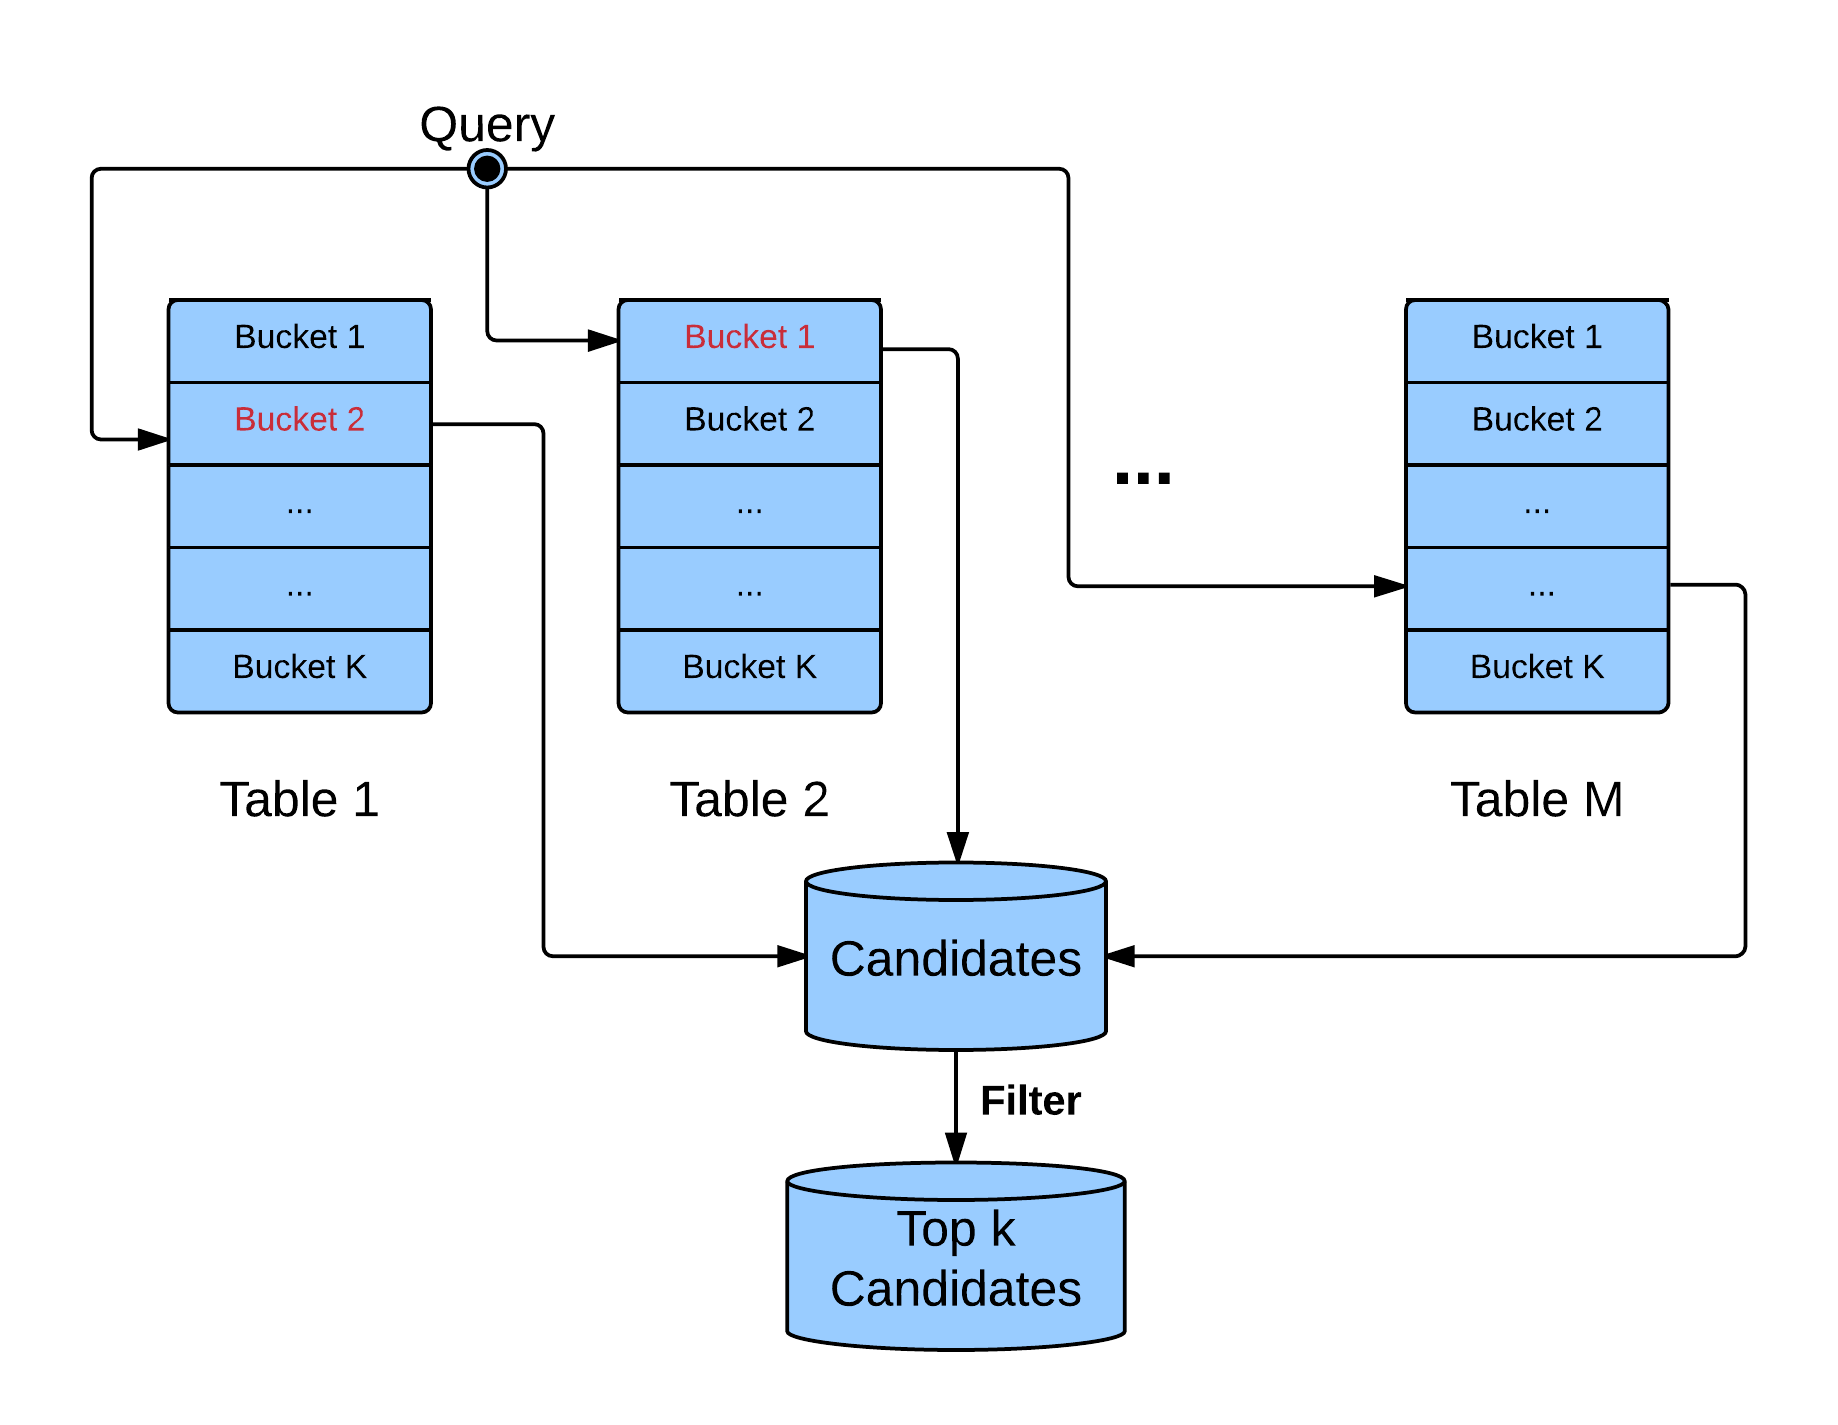
\includegraphics[width=8cm]{graph.png}`
	\vspace{-0.5cm}
	\caption{data processing pipeline of LSH}
	\label{figure:model-architecture}
	\vspace{-0.5cm}
\end{figure}

The psudocode of applying LSH-based KNN algorithm
for classification tasks can be viewed in \ref{classification}, which is widely applied in various areas: image recognition\cite{lee1991handwritten}, text classification\cite{tan2006effective}, intrusion detection\cite{liao2002use}, missing value estimation\cite{acuna2004treatment},  etc. 


\begin{algorithm}
	\SetKwInOut{Input}{Input}
	\SetKwInOut{Output}{Output}
	\underline{Function LSHkNN} $(H, Q, k)$\;
	\Input{Hash Table $H$, Query Data Set $Q$, and Neighbor Number $k$}
	\Output{Prediction List of labels $L$}
	$L \leftarrow \infty$
	
	\For(\tcp*[f]{for each query sample}){$q=1, 2, \ldots, n$ }{
		\For(\tcp*[f]{for each hash table}){$i=1, 2, \ldots, m$}{        
			compute $h_{q, i} = \mathsf{g}_i(Q_q)$ \\
			find candidates $C_i = findHash(H, h_{q, i})$
		}
		collect candidates C = $\bigcup\limits_{i=1}^{m} C_{i}$ \\

		\eIf{$length(C)\neq 0$}
		{
			find best candidates by some distance matric $C^{\prime} = findTop(C, min(k, length(C)))$ \\
			get the majority $l_q = \arg \max\limits_{c \in C^{\prime}} freq(label_c)$
			c
		}
		{
			$L.insert(lable_{random})$
		}
	}
	return $L$\;
		
	\caption{LSH-based Approximate k-Nearest Neighbor Search Algorithm}
	\label{classification}
\end{algorithm}

\subsection{Distributed LSH through Spark}
Note there are two points to optimize in the pipeline: batch-query 
and distributed hashing. First, each query is independent with others
so it is reasonable and practicable to compute them in a map-reduce way. 
Second, each hashing function is independently defined by randomly 
sampling $a, b$ and $w$, so we can apply the spark framework to 
parallel the iterative computation.

The psudocode of our distributed KNN algorithm implementation can be viewed in \ref{knn}.
Note two for-loops in the conventional version are fully adapted in the Apache Spark version. We will show this bring great value to the system especially when the data size, data dimension and 

\begin{algorithm}
	\SetKwInOut{Input}{Input}
	\SetKwInOut{Output}{Output}
	\underline{Function largeLSH} $(H, Q, k, d)$\;
	\Input{Hash Table $H$, Query Data Set $Q$, Neighbor Number $k$, and distance threshold $d$}
	\Output{Prediction List of labels $L$}
	generate ID column for $H$ and $Q$ \\
	results $\leftarrow$ H.approxSimilarityJoin(Q)  \tcp*[f]{search the hash table and union the results through a map-reduce way} \\
	resultsThres $\leftarrow$ filter(results, $d$) \tcp*[f]{get rid of candidates far from the query points}\\
	resultsSelected $\leftarrow$ \texttt{SELECT trainID, testID, distance FROM resultsThres} \\
	resultsPartitioned $\leftarrow$  findTopkByPartition(resultsSelected, $k$) \\
	$L$ $\leftarrow$ resultsPartitioned.map(groundtruthVector Intersect predictionVector)
	
	return $L$\;

	\caption{Distributed LSH}
	\label{knn}
\end{algorithm}

\section{Experimental Setup}

\subsection{Data}
\subsubsection{MNIST}
The MNIST database\footnote{\url{http://yann.lecun.com/exdb/mnist/}} of handwritten digits has a training set of 60,000 examples, and a test set of 10,000 examples, which is a subset of a larger set available from NIST. Each image is in the shape of $28 \times 28$ so the whole training and testing sets are in shape $60,000 \times 784$ and $10,000 \times 784$. The labels values are 0 to 9.
Many work has been tested with this training set and test set.

\subsubsection{SVHN}
SVHN\footnote{\url{http://ufldl.stanford.edu/housenumbers/}} is a real-world image dataset for developing machine learning algorithms with minimal requirement on data preprocessing and formatting. It can be seen as similar in flavor to MNIST (e.g., the images are of small cropped digits), but incorporates an order of magnitude more labeled data (over 600,000 digit images) and comes from a significantly harder, unsolved, real world problem (recognizing digits and numbers in natural scene images). 

\subsubsection{SIFT}
\cite{jegou2011product}

\subsection{Task}
\subsubsection{Nearest Neighbor Search}
\subsubsection{Image Classification}
\subsection{Parameters}
\subsubsection{Hardware Configuration}

We use Microsoft Azure HDInsight to create Spark clusters to run our 
experiment. For the horizontal scalability experiment we use a cluster consisting 
of two A3 head nodes with 4 cores, 7 GB RAM, and 285 GB of disk space per node and 
two A4 worker nodes with 8 cores, 14 GB RAM, and 605 GB of disk space per node. The 
A-series nodes are general purpose nodes. Each A3 node costs \$0.39/hour while each 
A4 node costs \$0.779/hour. \\

For running the SVHN and SIFT dataset experiments, we opted for a more powerful 
cluster powered by two D12 v2 head nodes with 4 cores, 28 GB RAM, and 200 GB of 
disk space per node and two two D13 v2 worker nodes with 8 cores, 56 GB RAM, and 
400 GB of disk space per node. The Dv2-series nodes are optimized nodes with the 
latest generation of CPUs. Each D12 v2 node costs \$0.925/hour while each D13 v2 
node costs \$1.664/hour. \\

For each particular experiment we vary number of executors, cores per executor, and 
memory per executor used by Spark. We indicate those in the relevant section.

\subsubsection{Parameters for LSH}
\subsubsection{Parameters for ANN-based Classification}

\section{Results}

First we summarize the results of our horizontal scalability test.

\section{Summary}


\section{Conclusion}

\section*{Acknowledgement}
We thank Professor Samer Al-Kiswany for helpful discussions regarding the direction 
of the project. We thank Microsoft for graciously providing Azure credits for 
Zhucheng Tu to use for his courses.
{\footnotesize \bibliographystyle{acm}
\bibliography{bibliography.bib}}

\end{document}







